\subsection{Number of Athletes by Age}\label{subsec:number-of-athletes-by-age}

To determine to determine the average age of the athletes, we can run the following SQL query:

\begin{minted}{sql}
SELECT AVG(age(birthdate))
FROM annp_final.athlete;
\end{minted}

From this, we can see that the average age of the athletes is 46 years, 6 months and 31 days.

We can also determine who's the youngest athlete by running the following SQL query:

\begin{minted}{sql}
SELECT *
FROM annp_final.athlete
ORDER BY age(birthdate) ASC
LIMIT 1;
\end{minted}

\begin{itemize}
    \item \textbf{Name:} Ana Mónica Eloi
    \item \textbf{Gender:} F
    \item \textbf{Birthdate:} 29/12/1996
    \item \textbf{Age:} 25 years
\end{itemize}

On the other hand, we can learn information about the oldest athlete by running the following SQL query:

\begin{minted}{sql}
SELECT *
FROM annp_final.athlete
ORDER BY age(birthdate) DESC
LIMIT 1;
\end{minted}

\begin{itemize}
    \item \textbf{Name:} Virgílio Zacarias Costa
    \item \textbf{Gender:} M
    \item \textbf{Birthdate:} 21/07/1931
    \item \textbf{Age:} 90 years
\end{itemize}

Finally, to determine the number of athletes by age, we can run the following SQL query using the PostgreSQL's built-in
\texttt{age} function:

\begin{minted}{sql}
SELECT COUNT(*), EXTRACT(YEAR FROM age(birthdate)) AS age
FROM annp_final.athlete
GROUP BY age
ORDER BY age ASC;
\end{minted}

We can then plot the result, as illustrated in \cref{fig:athletesbynation}.

\begin{figure}[H]
    \centering
    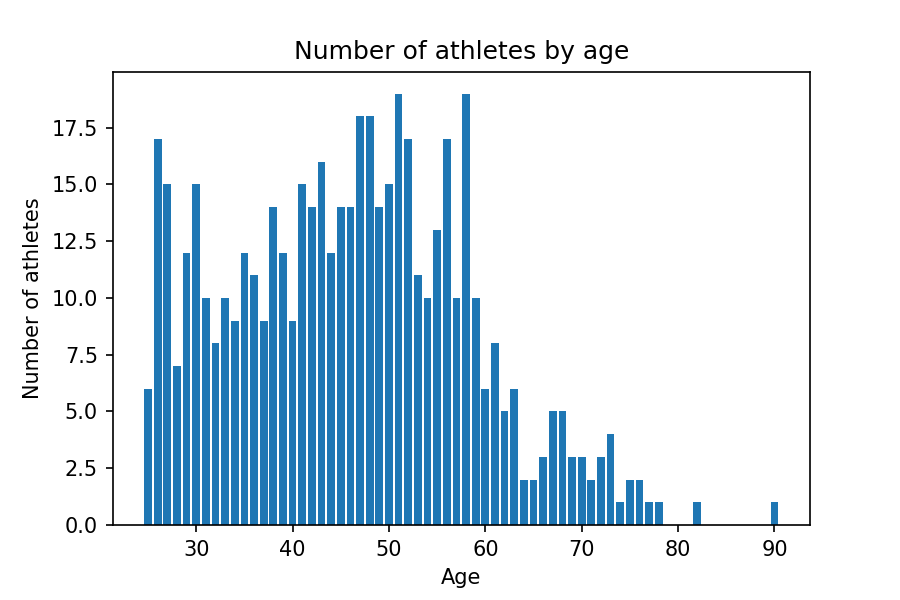
\includegraphics[width=\textwidth]{img/athletesbyage}
    \caption{Number of athletes by age}
    \label{fig:athletesbyage}
\end{figure}

\subsection{Number of Athletes by Nation}\label{subsec:number-of-athletes-by-nation}

To determine the number of athletes by nation, we can run the following SQL query:

\begin{minted}{sql}
SELECT COUNT(*) nationCount, nation
FROM annp_final.athlete
GROUP BY nation
ORDER BY nationCount ASC;
\end{minted}

We can then plot the result, as illustrated in \cref{fig:athletesbynation}.

\begin{figure}[H]
    \centering
    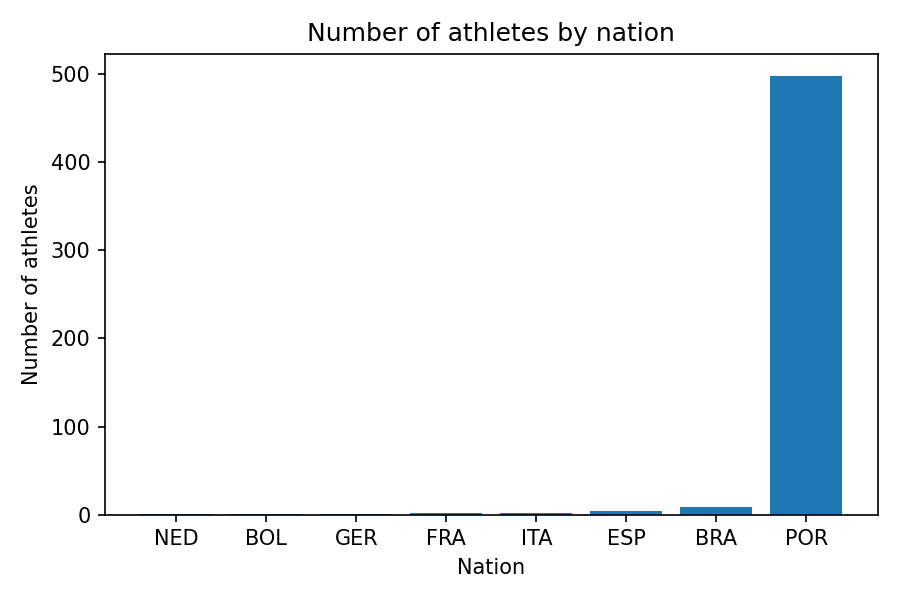
\includegraphics[width=.8\textwidth]{img/athletesbynation}
    \caption{Number of athletes by nation}
    \label{fig:athletesbynation}
\end{figure}

To have another perspective, we can also plot in a pie chart, as illustrated in \cref{fig:athletesbynation-pie}.

\begin{figure}[H]
    \centering
    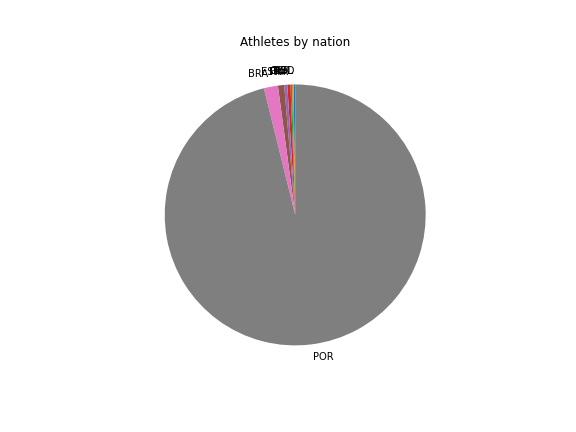
\includegraphics[width=.8\textwidth]{img/athletesbynation-piechart}
    \caption{Number of athletes by nation}
    \label{fig:athletesbynation-pie}
\end{figure}

\subsection{Number of Athletes by Gender}\label{subsec:number-of-athletes-by-gender}

To determine the number of athletes by gender, we can run the following SQL query:

\begin{minted}{sql}
SELECT COUNT(*), gender
FROM annp_final.athlete
GROUP BY gender;
\end{minted}

We can then plot the result, as illustrated in \cref{fig:athletesbygender}.

\begin{figure}[H]
    \centering
    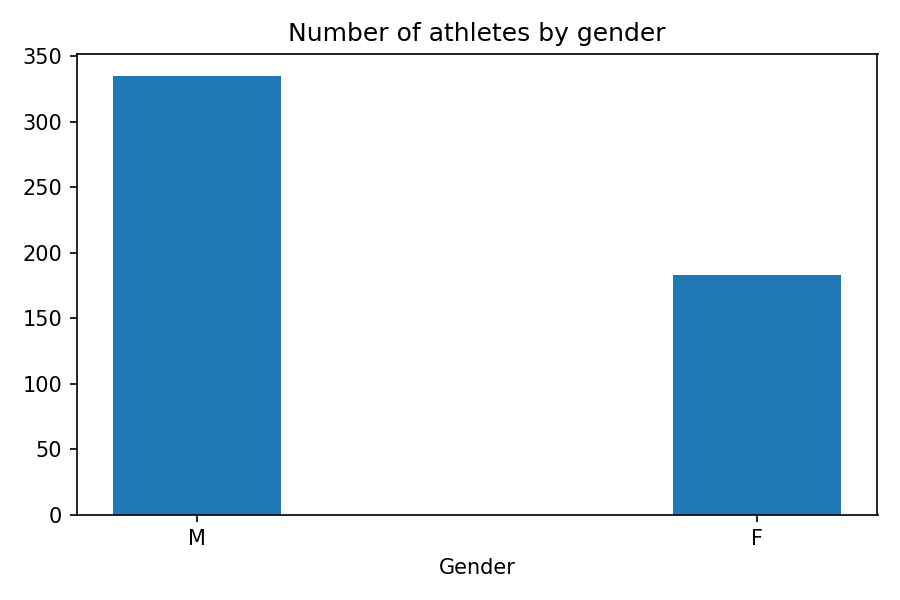
\includegraphics[width=.35\textwidth]{img/athletesbygender}
    \caption{Number of athletes by gender}
    \label{fig:athletesbygender}
\end{figure}

We can also plot this in a pie chart, as illustrated in \cref{fig:athletesbygender-pie}.

\begin{figure}[H]
    \centering
    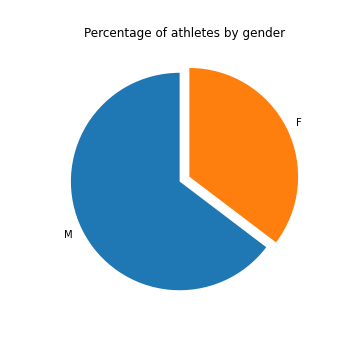
\includegraphics[width=.45\textwidth]{img/athletesbygender-pie}
    \caption{Percentage of athletes by gender}
    \label{fig:athletesbygender-pie}
\end{figure}

\subsection{Number of Events by Gender}\label{subsec:number-of-events-by-gender}

To determine the number of events by gender, we can run the following SQL query:

\begin{minted}{sql}
SELECT COUNT(*), gender
FROM annp_final.event
GROUP BY gender;
\end{minted}

We can then plot the result, as illustrated in \cref{fig:eventsbygender}.

\begin{figure}[H]
    \centering
    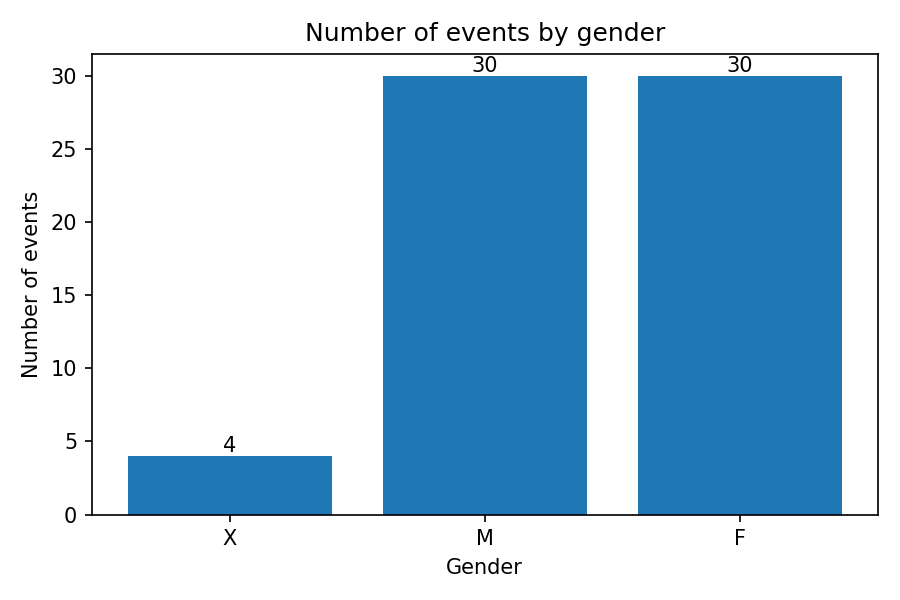
\includegraphics[width=.35\textwidth]{img/eventsbygender}
    \caption{Number of events by gender}
    \label{fig:eventsbygender}
\end{figure}

Here, the value \texttt{X} refers to events that allow athletes from both genders to participate.
We can also plot this in a pie chart, as illustrated in \cref{fig:eventsbygender-pie}.

\begin{figure}[H]
    \centering
    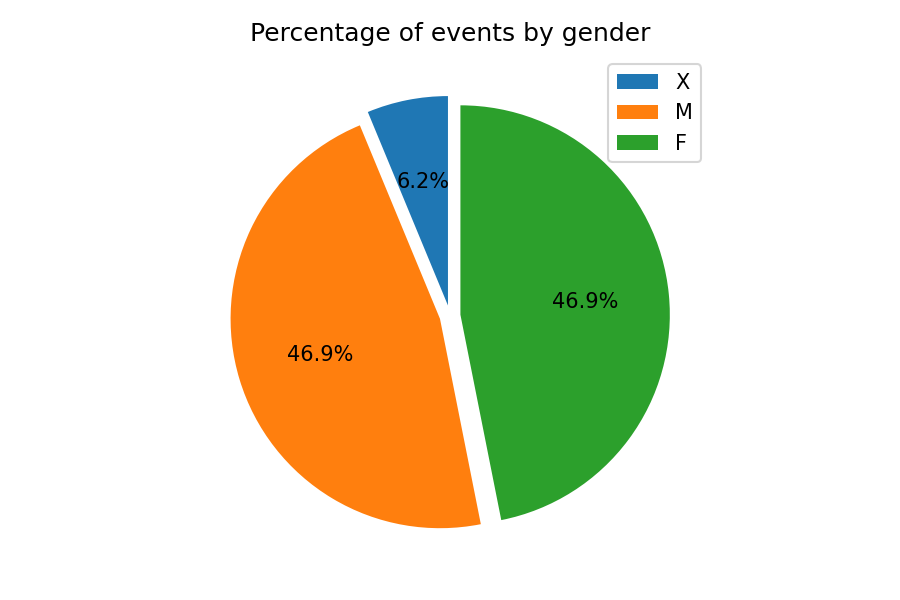
\includegraphics[width=.45\textwidth]{img/eventsbygender-pie}
    \caption{Percentage of events by gender}
    \label{fig:eventsbygender-pie}
\end{figure}

\subsection{Number of Clubs by Nation}\label{subsec:number-of-clubs-by-nation}

We can determine the number of clubs by each nation by running the following SQL query:

\begin{minted}{sql}
SELECT nation, COUNT(*) AS nationCount
FROM annp_final.club
GROUP BY nation
ORDER BY nationCount ASC;
\end{minted}

\textcolor{red}{COMPLETAR COM TEXTO}.

\begin{figure}[H]
    \centering
    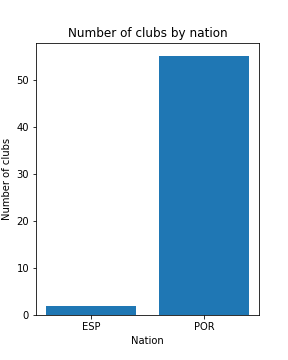
\includegraphics[width=.35\textwidth]{img/clubsbynation}
    \caption{Number of clubs by nation}
    \label{fig:clubs-by-nation}
\end{figure}

\textcolor{red}{COMPLETAR COM TEXTO}.

\begin{figure}[H]
    \centering
    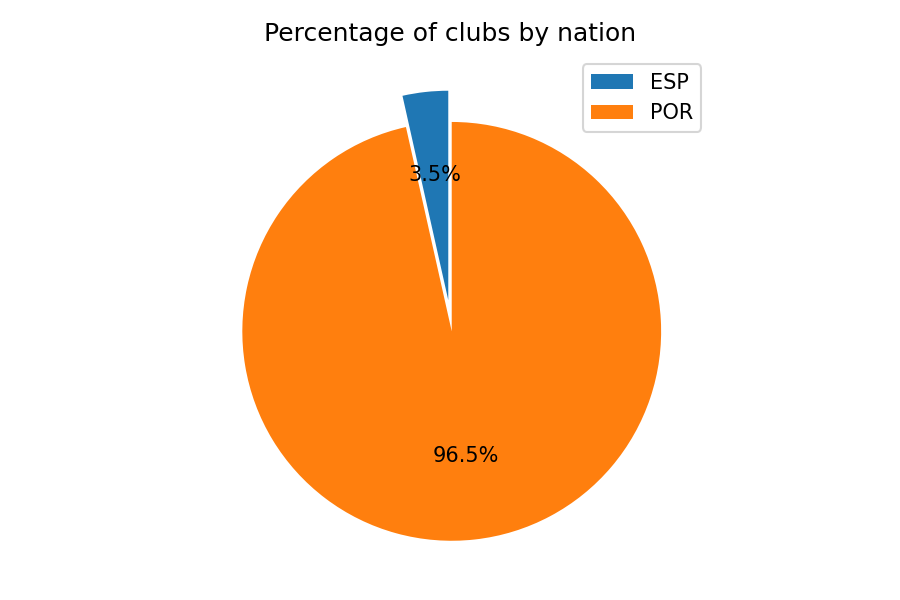
\includegraphics[width=.45\textwidth]{img/clubsbynation-pie}
    \caption{Percentage of clubs by nation}
    \label{fig:clubs-by-nation-pie}
\end{figure}

\subsection{Number of Clubs by Region}\label{subsec:number-of-clubs-by-region}

\textcolor{red}{COMPLETAR COM TEXTO}.

\begin{minted}{sql}
SELECT region, COUNT(*) AS regionCount
FROM annp_final.club
WHERE region SIMILAR TO '[A-Z]+'
GROUP BY region
ORDER BY regionCount ASC;
\end{minted}

\textcolor{red}{COMPLETAR COM TEXTO}.

\begin{figure}[H]
    \centering
    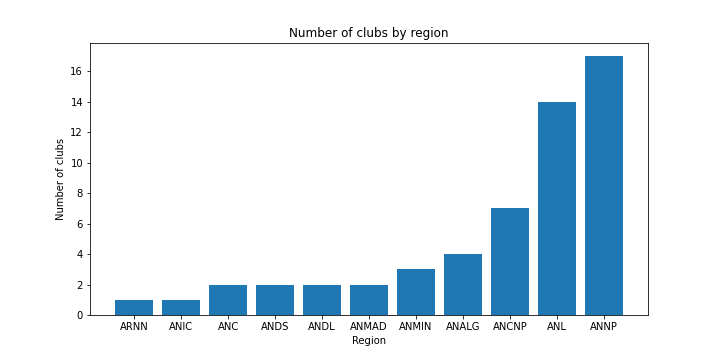
\includegraphics[width=.85\textwidth]{img/clubsbyregion}
    \caption{Number of clubs by region}
    \label{fig:clubs-by-region}
\end{figure}

\subsection{Swim Styles}

\textcolor{red}{COMPLETAR COM TEXTO (style com mais distance) É FRESSTYLE}.

\begin{minted}{sql}
SELECT *
FROM annp_final.swimstyle
ORDER BY distance DESC
LIMIT 1;
\end{minted}

\textcolor{red}{COMPLETAR COM TEXTO (style com menos distance) FLY}.

\begin{minted}{sql}
SELECT *
FROM annp_final.swimstyle
ORDER BY distance ASC
LIMIT 1;
\end{minted}

\subsection{Results}

\subsubsection{Average Swim Time}

\textcolor{red}{COMPLETAR COM TEXTO (resultado = 00:02:23.769068)}.

\begin{minted}{sql}
SELECT AVG(swimtime)
FROM annp_final.result;
\end{minted}

\subsubsection{Average Number of Points}

\textcolor{red}{COMPLETAR COM TEXTO (resultado = 340)}.
\begin{minted}{sql}
SELECT AVG(points)::numeric(10, 1)
FROM annp_final.result;
\end{minted}
